\documentclass[journal,comsoc]{IEEEtran}

\usepackage[T1]{fontenc}% optional T1 font encoding
\usepackage{cite}
\usepackage[pdftex]{graphicx}
\usepackage{epstopdf}
\usepackage{amsmath}
\usepackage[caption=false,font=footnotesize]{subfig}
\newcommand{\hbAverage}[1]{\overline{#1}}
\newcommand{\etal}{et al. }
\newcommand{\hbie}{i.e.,}
\newcommand{\hbeg}{e.g.,}
\newcommand{\hbSection}[1]{\section{#1}}
\newcommand{\hbQuote}[1]{``\textsf{{\footnotesize #1}}''}
\usepackage{color}
\newcommand{\hbIdea}[1]{{\color{red}{\scriptsize [{#1}]}}}
\newcommand{\myFigWidth}{8cm}
\usepackage[hidelinks]{hyperref}
\newcommand{\reffig}[1]{Fig.~\ref{#1}}
\newcommand{\refeq}[1]{Eq.~\ref{#1}}
\newcommand{\reftbl}[1]{Table~\ref{#1}}
\newcommand{\refsec}[1]{Sec.~\ref{#1}}
\newcommand{\refthm}[1]{Theorem~\ref{#1}}
\newcommand{\refthmA}[2]{\refthm{#1}(\ref{#2}}
\newcommand{\reflem}[1]{Lemma~\ref{#1}}
\newcommand{\refdef}[1]{Definition~\ref{#1}}
\newcommand{\refexmp}[1]{Example~\ref{#1}}
\newcommand{\refitem}[1]{(\ref{#1})}
\newcommand{\refcite}[1]{ref~\cite{#1}}
\usepackage[iso]{datetime}
\newcommand{\hbNow}{--Draft-- v\today/\currenttime} % version


\hyphenation{op-tical net-works semi-conduc-tor}


\begin{document}


\title{
	Smart presentation of HTML pages
}

\author{Kerim Can Macit}
% \thanks{
% H.~O.~Bingol  and Omer Basar are with 
% the Department of Computer Engineering, 
% Bogazici University, 
% Istanbul,
% 34342 Turkey 
% e-mail: bingol@boun.edu.tr.
% }% <-this % stops a space
% \thanks{Manuscript received December 1, 2015; revised XX XX, 2015.}}


\maketitle


% \begin{abstract}
% 	ABSTRACT WILL BE HERE
% \end{abstract}


% \begin{IEEEkeywords}
% 	HTML,
% 	Presentation,
% 	Markdown
% \end{IEEEkeywords}


\IEEEpeerreviewmaketitle


\section{Introduction}

\IEEEPARstart{T}{here} 
%Using 
are several options and plenty of dedicated software for generating presentations, from Microsoft PowerPoint to web services, like Prezi. Each option has some advantages and disadvantages over others. In this project, I will research on HTML page usage for presentation and implement navigation handler for presentation purposes.

HTML pages for presentation has some advantages over traditional presentation software. The most dominant advantage of HTML presentation is that it does not require any special software in order to present. Any device with basic internet browser will be able to handle HTML presentation which makes it platform independent. 

HTML pages also give more flexibility compared to traditional ones. Also, most popular presentation programs requires subscription in order to use. Also, with some programming knowledge, structure and navigation tool can easily be change.

HTML pages are also tends to be smaller in size. Therefore, it has some advantage in publishing and sharing the presentation.

Although having some advantages, generating HTML pages for presentation requires some technical knowledge. Therefore, in this application, I will use some type of markdown to HTML converter in order to make it easy for the presenter or presentation generator.

% =========================================================================
\section{SYSTEM DESCRIPTION}

Basically, the system can be explained as HTML page presentation app. App has 3 main features, mark-down to HTML generator, presentation ordering part and lastly navigation system.

The aim of MD to HTML converter is to make app easy-to-use. Expecting generating HTML pages in order to use the app creates conflicts because regular user with no technical knowledge found extremely hard generate HTML pages. In this application, instead of expecting pure HTML, MD can be used for generating the presentation page.

In the presentation ordering part, the user can select the order of presentation using already generated HTML pages. With this feature, user can reuse HTML pages in more than one presentation without requiring to copying. 

Lastly, the app has navigation system which is used to present the pages in ordered way or go to selected presentation page using table of content page. The system may also include timer to move automatically next slide.

% =========================================================================
\section{Requirements}

Requirements will be here

\section{System Design}
System Design goes here.

\href{http://www.google.de}{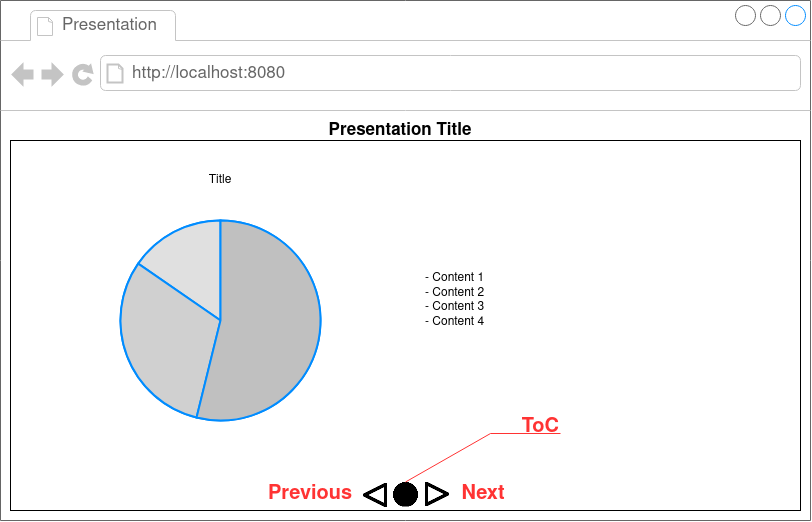
\includegraphics[scale=0.33]{Mockups/NavigationSystem_1.png}} % [1]

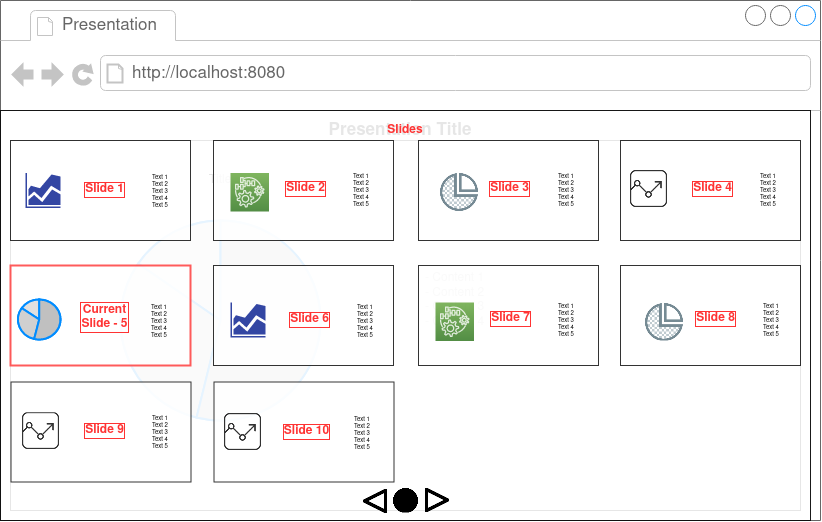
\includegraphics[scale=0.33]{Mockups/NavigationSystem_2.png}

\section{Implementation}
Implementation goes here.

\section{Demonstration}
Demonstration will be here.

\section{Conclusion}
The conclusion will be here.


\appendices
\section{Proof of the First Zonklar Equation}
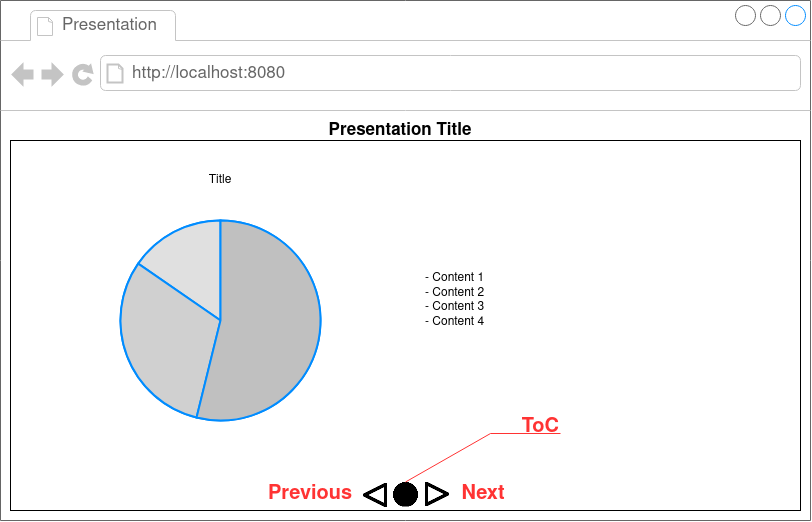
\includegraphics[scale=0.2]{Mockups/NavigationSystem_1.png}

% Proof of the First Zonklar Equation


% use section* for acknowledgment
% \section*{Acknowledgment}


% The authors would like to thank...


\ifCLASSOPTIONcaptionsoff
  \newpage
\fi

\IEEEtriggeratref{32}
\bibliographystyle{IEEEtran}
\bibliography{IEEEabrv,bingol-PaperTemplateIEEE}

\end{document}


